% Version 3 December 2023
% See section 11 of the User Manual for version history
%
%%%%%%%%%%%%%%%%%%%%%%%%%%%%%%%%%%%%%%%%%%%%%%%%%%%%%%%%%%%%%%%%%%%%%%
%%                                                                 %%
%% Please do not use \input{...} to include other tex files.       %%
%% Submit your LaTeX manuscript as one .tex document.              %%
%%                                                                 %%
%% All additional figures and files should be attached             %%
%% separately and not embedded in the \TeX\ document itself.       %%
%%                                                                 %%
%%%%%%%%%%%%%%%%%%%%%%%%%%%%%%%%%%%%%%%%%%%%%%%%%%%%%%%%%%%%%%%%%%%%%

% \documentclass[referee,sn-basic]{sn-jnl}% referee option is meant for double line spacing

%%=======================================================%%
%% to print line numbers in the margin use lineno option %%
%%=======================================================%%

% \documentclass[lineno,sn-basic]{sn-jnl}% Basic Springer Nature Reference Style/Chemistry Reference Style

%%======================================================%%
%% to compile with pdflatex/xelatex use pdflatex option %%
%%======================================================%%

% \documentclass[pdflatex,sn-basic]{sn-jnl}% Basic Springer Nature Reference Style/Chemistry Reference Style

%%Note: the following reference styles support Namedate and Numbered referencing. By default the style follows the most common style. To switch between the options you can add or remove “Numbered” in the optional parenthesis.\\

%%The option is available for: sn-basic.bst, sn-vancouver.bst, sn-chicago.bst%

\documentclass[pdflatex,sn-nature, lineno]{sn-jnl}% Style for submissions to Nature Portfolio journals
% \documentclass[pdflatex,sn-basic]{sn-jnl}% Basic Springer Nature Reference Style/Chemistry Reference Style
% \documentclass[pdflatex, sn-mathphys-num, lineno]{sn-jnl}% Math and Physical Sciences Numbered Reference Style
%%\documentclass[pdflatex,sn-mathphys-ay]{sn-jnl}% Math and Physical Sciences Author Year Reference Style
%%\documentclass[pdflatex,sn-aps]{sn-jnl}% American Physical Society (APS) Reference Style
%%\documentclass[pdflatex,sn-vancouver,Numbered]{sn-jnl}% Vancouver Reference Style
%%\documentclass[pdflatex,sn-apa]{sn-jnl}% APA Reference Style
%%\documentclass[pdflatex,sn-chicago]{sn-jnl}% Chicago-based Humanities Reference Style

%%%% Standard Packages
%% additional latex packages if required can be included here>
\usepackage{graphicx}%
\usepackage{multirow}%
\usepackage{amsmath,amssymb,amsfonts}%
\usepackage{amsthm}%
\usepackage{mathrsfs}%
\usepackage[title]{appendix}%
\usepackage{xcolor}%
\usepackage{textcomp}%
\usepackage{manyfoot}%
\usepackage{booktabs}%
\usepackage{algorithm}%
\usepackage{algorithmicx}%
\usepackage{algpseudocode}%
\usepackage{listings}%

\usepackage{xspace}
\usepackage{standalone}

%% my package start
% for the command \hl
\usepackage{soul}
\usepackage{titlesec}


% for collabration and will remove before submit
\newcommand{\yy}[1]{\textcolor{cyan}{\textbf{[Yangyang: #1]}}}
\newcommand{\rd}[1]{\textcolor{green}{\textbf{[Dr.Yang: #1]}}}
\newcommand{\ty}[1]{\textcolor{orange}{\textbf{[Tingyou: #1]}}}
\newcommand{\qx}[1]{\textcolor{purple}{\textbf{[Qingxiang: #1]}}}

% for collabration and will remove before submit

% \usepackage{caption}
% \usepackage{subfig}
\usepackage{enumitem}

\usepackage[detect-all=true]{siunitx}
\sisetup{
    scientific-notation=false,
    round-mode = places,
    round-precision = 0
}

\usepackage[acronym, automake, style=index, shortcuts]{glossaries-extra}
\setabbreviationstyle[acronym]{long-short}
% define glossaries
\makeglossaries

\newacronym{blat}{BLAT}{BLAST-like alignment tool}
\newacronym{llm}{LLM}{Large Language Model}
\newacronym{hmm}{HMM}{Hidden Markov Model}
\newacronym{gpu}{GPU}{Graphics Processing Unit}
\newacronym{hpc}{HPC}{High Performance Computing}
\newacronym{bert}{BERT}{Bidirectional Encoder Representations from Transformers}
\newacronym{gpt}{GPT}{Generative Pre-trained Transformer}

\newacronym{ide}{IDE}{Integrated Development Environment}
\newacronym{cd}{CD}{Continuous Development}
\newacronym{ucsc}{UCSC}{UCSC Genome Browser}
\newacronym{glm}{GLM}{Genomic Language Model}
\newacronym{lcglm}{LCGLM}{long-context genomic language model}
\newacronym{snp}{SNP}{Single Nucleotide Polymorphism}
\newacronym{fm}{FM}{Foundational Model}
\newacronym{nlp}{NLP}{Natural Language Processing}

\newacronym{mlp}{MLP}{multilayer perceptron}
\newacronym{drs}{dRNA-seq}{direct RNA sequencing}
\newacronym{ont}{ONT}{Oxford Nanopore Technologies}
\newacronym{pb}{PacBio}{Pacific Biosciences}

\newacronym{go}{GO}{Gene Ontology}
\newacronym{pcr}{PCR}{Polymerase Chain Reaction}

\newacronym{fsm}{FSM}{Full splice match}
\newacronym{ism}{ISM}{Incomplete splice match}
\newacronym{nic}{NIC}{Novel in catalog}
\newacronym{nnc}{NNC}{Novel not in catalog}

\newacronym{tp}{TP}{True Positive}
\newacronym{fp}{FP}{False Positive}
\newacronym{fn}{FN}{False Negative}

\newacronym{mrna}{mRNA}{messenger RNA}
\newacronym{rta}{RTA}{reverse transcriptase adapter}
\newacronym{sgnex}{SG-NEx}{Singapore Nanopore Expression Project}
\newacronym{lrgasp}{LRGASP}{Long-read RNA-Seq Genome Annotation Assessment Project}
\newacronym{atcc}{ATCC}{American Type Culture Collection}
\newacronym{ccle}{CCLE}{Cancer Cell Line Encyclopedia}
\newacronym{david}{DAVID}{Database for Annotation, Visualization, and Integrated Discovery}
\newacronym{geo}{GEO}{Gene Expression Omnibus}

\newcommand{\figref}[2]{Fig.~\hyperref[#1]{\ref*{#1}#2}}
\newcommand{\edfigref}[2]{Extended Data Fig.~\hyperref[#1]{\ref*{#1}#2}}
\newcommand{\edtableref}[2]{Extended Data Table~\hyperref[#1]{\ref*{#1}#2}}
\newcommand{\edfigrefrg}[3]{Extended Data Fig.~\hyperref[#1]{\ref*{#1}#2-\ref*{#1}#3}}

\graphicspath{{../figures}}
%% my package end


%%%%%=============================================================================%%%%
%%%%  Remarks: This template is provided to aid authors with the preparation
%%%%  of original research articles intended for submission to journals published
%%%%  by Springer Nature. The guidance has been prepared in partnership with
%%%%  production teams to conform to Springer Nature technical requirements.
%%%%  Editorial and presentation requirements differ among journal portfolios and
%%%%  research disciplines. You may find sections in this template are irrelevant
%%%%  to your work and are empowered to omit any such section if allowed by the
%%%%  journal you intend to submit to. The submission guidelines and policies
%%%%  of the journal take precedence. A detailed User Manual is available in the
%%%%  template package for technical guidance.
%%%%%=============================================================================%%%%

%% as per the requirement new theorem styles can be included as shown below
%\theoremstyle{thmstyleone}%
%\newtheorem{theorem}{Theorem}%  meant for continuous numbers
%%\newtheorem{theorem}{Theorem}[section]% meant for sectionwise numbers
%% optional argument [theorem] produces theorem numbering sequence instead of independent numbers for Proposition
%\newtheorem{proposition}[theorem]{Proposition}%
%%\newtheorem{proposition}{Proposition}% to get separate numbers for theorem and proposition etc.

%\theoremstyle{thmstyletwo}%
%\newtheorem{example}{Example}%
%\newtheorem{remark}{Remark}%

%\theoremstyle{thmstylethree}%
%\newtheorem{definition}{Definition}%

\raggedbottom
\unnumbered% uncomment this for unnumbered level heads

\begin{document}

\title[Article Title]{Genomic Language Model Mitigates Chimera Artifacts in Nanopore Direct RNA Sequencing}

%%=============================================================%%
%% GivenName	-> \fnm{Joergen W.}
%% Particle	-> \spfx{van der} -> surname prefix
%% FamilyName	-> \sur{Ploeg}
%% Suffix	-> \sfx{IV}
%% \author*[1,2]{\fnm{Joergen W.} \spfx{van der} \sur{Ploeg}
%%  \sfx{IV}}\email{iauthor@gmail.com}
%%=============================================================%%

\author[1]{\fnm{Yangyang} \sur{Li}}\email{yangyang.li@northwestern.edu}
\equalcont{These authors contributed equally to this work.}

% \author*[1,2]{\fnm{First} \sur{Author}}\email{iauthor@gmail.com}
\author[1]{\fnm{Ting-You} \sur{Wang}}\email{tywang@northwestern.edu}
\equalcont{These authors contributed equally to this work.}

\author[1]{\fnm{Qingxiang} \sur{Guo}}\email{qingxiang.guo@northwestern.edu}

\author[1]{\fnm{Yanan} \sur{Ren}}\email{ynren1020@gmail.com}
\author[1]{\fnm{Xiaotong} \sur{Lu}}\email{xiaotong.lu@northwestern.edu}

\author[1,2]{\fnm{Qi} \sur{Cao}}\email{qi.cao@northwestern.edu}
\author*[1,2]{\fnm{Rendong} \sur{Yang}}\email{rendong.yang@northwestern.edu}

\affil[1]{\orgdiv{Department of Urology}, \orgname{Northwestern University Feinberg School of Medicine}, \orgaddress{\street{303 E Superior St}, \city{Chicago}, \postcode{60611}, \state{IL}, \country{USA}}}
\affil[2]{\orgdiv{Robert H. Lurie Comprehensive Cancer Center}, \orgname{Northwestern University Feinberg School of Medicine}, \orgaddress{\street{675 N St Clair St}, \city{Chicago}, \postcode{60611}, \state{IL}, \country{USA}}}

% \author[1,2]{\fnm{Third} \sur{Author}}\email{iiiauthor@gmail.com}
% \equalcont{These authors contributed equally to this work.}

% \affil*[1]{\orgdiv{Department}, \orgname{Organization}, \orgaddress{\street{Street}, \city{City}, \postcode{100190}, \state{State}, \country{Country}}}
% \affil[2]{\orgdiv{Department}, \orgname{Organization}, \orgaddress{\street{Street}, \city{City}, \postcode{10587}, \state{State}, \country{Country}}}
% \affil[3]{\orgdiv{Department}, \orgname{Organization}, \orgaddress{\street{Street}, \city{City}, \postcode{610101}, \state{State}, \country{Country}}}

%%==================================%%
%% Sample for unstructured abstract %%
%%==================================%%

\abstract{
	Chimera artifacts in nanopore \gls{drs} introduce substantial inaccuracies, complicating downstream applications such as transcript annotation and gene fusion detection. Current basecalling models are unable to detect or mitigate these artifacts, limiting the reliability and utility of \gls{drs} for transcriptomics research. To address this challenge, we present DeepChopper, a genomic language model specifically designed to identify and remove adapter sequences from base-called \gls{drs} long reads with single-base precision. Operating independently of raw signal or alignment information, DeepChopper effectively eliminates chimeric read artifacts, significantly enhancing the accuracy of crucial downstream analyses. This improvement in reliability unlocks the full potential of nanopore \gls{drs}, establishing it as a more robust tool for diverse transcriptomics applications.
	%Chimera artifacts in nanopore \gls{drs} can significantly distort transcriptome analyses, yet their detection and removal remain challenging due to limitations in existing basecalling models. We present DeepChopper, a genomic language model that precisely identifies and removes adapter sequences from base-called \gls{drs} long reads at single-base resolution, operating independently of raw signal or alignment information to effectively eliminate chimeric read artifacts. By removing these artifacts, DeepChopper substantially improves the accuracy of critical downstream analyses, such as transcript annotation and gene fusion detection, thereby enhancing the reliability and utility of nanopore \gls{drs} for transcriptomics research.

	%	Nanopore \gls{drs} has transformed transcriptomics by enabling full-length RNA analysis in a single read, but its utility is hindered by chimera artifacts that compromise data quality. We introduce DeepChopper, a genomic large language model designed to process long-read nanopore \gls{drs} data by efficiently identifying and removing adapter sequences directly from base-called reads, without the need for raw signal or alignment data. DeepChopper leverages long-range dependency modeling and quality-aware processing, enabling it to achieve broad contextual understanding while maintaining single-nucleotide resolution. Applied across multiple cell lines and sequencing platforms, DeepChopper reduced chimeric read artifacts by up to 91\% and decreased false-positive gene fusion calls by 89\%. This enhanced accuracy significantly improved downstream analyses, including transcript annotation and gene fusion detection in cancer transcriptomes. Our findings demonstrate the potential of large language models to tackle complex biological data, offering a robust tool for advancing genomics and biotechnology applications.
}
\maketitle

\section{Introduction}

% Outline
% 1. Sequencing history
% 2. Genomics LLM history
% 3. Challenges of LLM / efficiency of transformer and improvements
% 3.1 long range
% 3.2 single nucleotide resolution
% 4. Cons of drs
% 5. Our method
% 6. Results
% 7. Conclusion

Long-read RNA sequencing technologies are revolutionizing transcriptomic research by providing unparalleled resolution for detecting complex splicing and gene fusion events often missed by conventional short-read RNA-seq methods.
Among these technologies, \gls{ont} \gls{drs} stands out by sequencing full-length RNA molecules directly, preserving native RNA modifications and allowing a more accurate and comprehensive analysis of RNA biology.
This approach bypasses the inherent limitations of cDNA-based sequencing methods, such as artifacts arising from reverse transcription, template switching, and \gls{pcr} amplification~\cite{garalde2018highly, jain2022advances}.

Despite these advantages, a critical question remains: Does \gls{ont} \gls{drs} introduce technical artifacts?
A previous study has suggested that \gls{drs} might generate chimera artifacts, leading to multi-mapped reads~\cite{smith2020molecular}.
These artifacts may result from ligation during library preparation or chimeric reads produced by software missing the open pore signal, potentially confounding downstream analyses such as transcriptome assembly, quantification, and detection of alternative splicing and gene fusion events.
Detecting these chimera artifacts is challenging because long-read aligners often produce chimeric alignments from such artifacts that are indistinguishable from those derived from true gene fusion events.
Importantly, chimeric read artifacts frequently contain internal adapter sequences~\cite{smith2020molecular}, which could theoretically serve as a distinguishing feature to differentiate them from true gene fusion-derived reads.
However, \gls{ont} \gls{drs} basecallers, trained in RNA, struggle to properly call these DNA-based adapter sequences under an RNA model~\cite{liu2024sequencing}.
\hl{As a result, current adapter detection tools\mbox{~\cite{pychopper, Wick2017, bonenfant2023porechop}} cannot exploit this feature to eliminate chimeric read artifacts, leaving the issue unresolved} (\edtableref{tab:st1}{}).

To address these challenges, we developed DeepChopper, a \gls{glm} for long-read sequence analysis.
Leveraging recent advances in \gls{llm} that can interpret complex genetic patterns~\cite{benegas2024genomic}, DeepChopper processes long genomic contexts with single-nucleotide resolution.
This capability enables precise identification of \gls{ont} adapter sequences within base-called long reads, facilitating the detection and removal of chimeric read artifacts in \gls{drs} data.
Through analysis of both existing and newly generated \gls{drs} data, including those using the most recent RNA004 chemistry, we uncovered the prevalence of chimera artifacts—a critical issue previously overlooked in the long-read sequencing field.
We demonstrated that these artifacts significantly impact transcriptomic analysis by complicating gene fusion detection, transcript annotation, and alternative splicing studies.
By both identifying and addressing this problem, our work enhances the reliability and precision of \gls{drs} data, substantially improving its utility in transcriptomic research.

\section{Results and Discussion}

\subsection{DeepChopper Architecture and Training}

\begin{figure}[!ht]
	\includegraphics[height=0.63\columnwidth]{finals/figure1}
	\caption{{\bf DeepChopper architecture and methodology.} (a) Overview of the DeepChopper model. Raw sequences are first tokenized into vectors and processed by HyenaDNA to generate embedding features. These features are integrated with base quality information in the quality block to produce per-token probability scores. A refinement strategy further optimizes the predictions. Created with BioRender.com. (b) Architecture of the quality block. The block combines a \gls{mlp} (purple) with a residual connection to process both embedding features and sequence base quality scores (green vector). The output provides per-token probabilities indicating whether each base belongs to an adapter sequence. (c) Illustration of the sliding window refinement method. The model's initial predictions are inferred from probability. Then the predictions are processed using a sliding window approach (red rectangle) to refine predictions. The dashed rectangle highlights the first four steps of this refinement process, where each step refines the prediction for a single base position in terms of the majority vote.}\label{fig:f1}
\end{figure}

DeepChopper leverages the \gls{lcglm} HyenaDNA~\cite{nguyen2024hyenadna}, which excels at capturing long-range dependencies (\figref{fig:f1}{a}).
To address HyenaDNA's inability to process sequencing base quality information, DeepChopper extends its framework by incorporating a dedicated quality block, which is a neural network comprising multiple \glspl{mlp} with residual connections~\cite{he2015deep} (\figref{fig:f1}{b}, See \hyperref[sec:methods]{Methods} for details).
This addition enables the effective utilization of sequencing base quality, a crucial feature for improving prediction accuracy.
\hl{Our ablation study demonstrated a clear benefit from incorporating the quality block component into the model architecture.
	As shown in \mbox{\edtableref{tab:st2}{}}, models with the quality block achieved an F1 score of 0.99, compared to 0.97 for models without this component.}
By combining broad contextual understanding with nucleotide-level precision~\cite{poli2023hyena}, this hybrid architecture allows DeepChopper to accurately identify and process adapters sequences.
Reads containing internal adapters are split into multiple records, with $3'$ end adapters simultaneously trimmed (\figref{fig:f1}{a}), thereby preserving authentic biological sequences and eliminating chimera artifacts.

To further refine the prediction accuracy, DeepChopper implements a post-processing stage using a sliding window and majority vote approach, as illustrated in~\figref{fig:f1}{c}.
The model applies sliding window with a stride of 1 across the read, analyzing the distribution of predicted adapter positions within each window (See \hyperref[sec:methods]{Methods} for details).
This refinement process ensures that the predicted adapter sequences are contiguous and biologically plausible by smoothing irregularities and eliminating isolated false positives, while preserving genuine adapter signals that demonstrate consistent patterns across adjacent windows.
By applying this iterative refinement strategy, DeepChopper is able to optimize the final predictions and improve the overall accuracy of the adapter detection.


\hl{Comparing to existing general-purpose GLM, DeepChopper is specifically optimized for long-read sequence analysis with single-nucleotide resolution.
	This fine-grained resolution represents a critical advantage for genomic analysis tasks requiring precise base-level predictions.
	While DNABERT\mbox{~\cite{ji2021dnabert}} is limited to approximately 512 bp, DNABERT2\mbox{~\cite{zhou2023dnabert2}} to 10,000 bp, and Nucleotide Transformer\mbox{~\cite{dalla2024nucleotide}} to 6,000 bp, DeepChopper processes sequences up to 32 kilobases—a context length sufficient to capture most complete mRNA transcripts.}
This extended sequence capacity, combined with single-nucleotide tokenization, enables DeepChopper to precisely identify non-reference elements such as \gls{ont} adapters with base-pair accuracy, a critical advantage for detecting chimeric artifacts in \gls{drs} sequencing data.
Its efficient architecture, comprising just 4.6 million parameters, makes DeepChopper computationally practical for large-scale \gls{drs} analysis, unlike resource-intensive models such as Evo~\cite{nguyen2024sequence}, which requires billions of parameters.
This combination of long context processing, high-resolution accuracy, and computational efficiency makes DeepChopper particularly well-suited for analyzing massive long-read sequences (\edtableref{tab:st2}{}).

% Result
\begin{figure}[!ht]
	\includegraphics[height=0.6\columnwidth]{finals/figure2}
	\caption{{\bf Detection of chimeric read artifacts in \gls{drs} data using DeepChopper and validation with orthogonal sequencing platforms}  (a) Length distribution of predicted adapters by DeepChopper in VCaP \gls{drs} data. (b) Distribution of relative adapter position along read length in VCaP \gls{drs} data. Grey rectangle represents a long read from $5'$ to $3'$. Relative position is calculated as the ratio of the length before DeepChopper predicted adapter start position to the total read length. (c) Distribution of segments per read after trimming: 1 segment indicates $3'$ end adapter trimmed, while 2 or more indicate internal adapters trimmed. (d) Chimeric alignments (in thousands) for VCaP \gls{drs} reads processed by Dorado with and without adapter trimming, and DeepChopper. DeepChopper greatly reduces chimeric alignments not supported by direct cDNA sequencing. (e) Distribution of base qualities from identified internal adapters by DeepChopper. Background colors indicate quality levels: green (high), yellow (medium), and red (low). (f) \gls{blat} identity distribution of the internal adapter sequences mapping against human reference genome. (g) The number of chimeric alignments (in thousands) for A549, HCT116, HepG2, K562, and MCF7 cell lines processed by Dorado with adapter trimming and DeepChopper. DeepChopper consistently reduces chimeric alignments not supported by cDNA sequencing across all cell lines. (h) Chimeric alignments from \gls{drs} of the WTC11 cell line, evaluated for support using additional \gls{ont} and \gls{pb} sequencing data with different protocols. DeepChopper reduces unsupported chimeric alignments across all methods compared to Dorado with adapter trimming.}\label{fig:f2}
\end{figure}

To train DeepChopper for identifying adapter sequences within \gls{drs} long reads, we utilized data from six human cell lines: HEK293T, A549, HCT116, HepG2, K562 and MCF-7 provided by the \gls{sgnex}~\cite{chen2021systematic}.
We curated a training set of 540,000 long reads initially deemed free of adapters and inserted putative adapter sequences, derived from the raw \gls{drs} data, into these reads to create instances containing internal and $3'$ end adapters (See \hyperref[sec:methods]{Methods} for details).
An independent test set comprising 60,000 long reads was held out for performance evaluation.
DeepChopper achieved recall, precision, and F1 scores above 0.99 (\edfigref{fig:sf1}{}), demonstrating its high accuracy in detecting adapter sequences.
\hl{The benchmarking results clearly demonstrate that existing adapter trimming tools\mbox{~\cite{pychopper, Wick2017, bonenfant2023porechop}} fail to identify adapter sequences in \mbox{\gls{drs}} data.}


\hl{Our model demonstrated exceptional binary classification performance in differentiating adapter from non-adapter sequences at single base pair resolution when evaluated on the independent test set.
	\mbox{\edfigref{fig:adaprob}{}}  illustrates the probability distributions of model predictions on this held-out data, stratified by ground truth labels.
	For true adapter base pairs (\mbox{\edfigref{fig:adaprob}{a}}), the model assigned high probabilities ($>0.8$) to the adapter class, while confidently predicting low probabilities ($<0.2$) for the non-adapter class.
	Conversely, for true non-adapter base pairs (\mbox{\edfigref{fig:adaprob}{b}}), the model correctly assigned high probabilities ($>0.8$) to the non-adapter class and low probabilities ($<0.2$) to the adapter class.
	The strongly bimodal nature of these distributions on unseen test data, with minimal intermediate probability values, indicates the model's decisive classification capabilities at single-nucleotide resolution with little uncertainty between classes, suggesting robust feature extraction, decision boundary formation during training, and excellent generalization to independent samples.}

To further assess DeepChopper’s ability to detect chimera artifacts in real data, we generated an additional \gls{drs} dataset using the prostate cancer VCaP cell line, which was not included in the training data.
This independent dataset provides a robust framework for evaluating chimera artifacts in genuine \gls{drs} samples, ensuring that DeepChopper's performance generalizes beyond the training data.


% For the specific subsection you want to highlight:
%{
%    \titleformat{\subsection}
%    {\normalfont\large\bfseries}
%    {\thesubsection}
%    {1em}
%    {\colorbox{yellow}}  % This highlights the subsection title

%\subsection{Runtime Performance and Resource Utilization}
%\subsection{DeepChopper Pipeline and Computational Performance}
%}

\subsection{Chimeric Read Artifact Detection}

We conducted \gls{drs} of VCaP cells using \gls{ont}'s SQK-RNA002 chemistry, consistent with the \gls{sgnex} project. Using a MinION sequencer with four R9.4 flow cells, we generated 9,177,639 long reads in FASTQ format, with base-calling performed by \gls{ont}'s Dorado software~\cite{dorado2023}.

\hl{DeepChopper was then applied for adapter trimming and correction of chimeric read artifacts. To enhance computational efficiency, DeepChopper employs a three-stage pipeline: (1) FASTQ inputs are converted to the Parquet format for optimized data access, (2) a neural network model predicts adapter sequences, and (3) post-processing refines these predictions. Key optimizations include implementing computationally intensive components in Rust, leveraging GPU acceleration for neural network inference, and parallelizing pre- and post-processing operations.}


\hl{We evaluated the computational performance of our pipeline using sequencing data from the VCaP cell line at various sampling depths.
	\mbox{\edfigref{fig:sf2a}{}} illustrates the runtime and memory requirements across different data sizes (0.1M, 0.5M, 1M reads, and the full dataset (9M)).
	As shown in \mbox{\edfigref{fig:sf2a}{a}}, the total processing time increased non-linearly with data size, from approximately 0.1 hours for the smallest sample (0.1M) to 5 hours for the full dataset.
	The prediction stage emerged as the primary computational bottleneck, accounting for over 70\% of the total runtime in the full dataset.
	FASTQ conversion and post-processing times also increased with data size but remained relatively modest compared to the prediction stage.
	Memory utilization (\mbox{\edfigref{fig:sf2a}{b}}) demonstrated similar scaling patterns with increasing data size.
	The prediction stage on CPU required the highest memory resources, approaching 70GB for the 1M and full datasets.
	Notably, GPU-based prediction consistently required less memory than its CPU counterpart across all data sizes, though the difference narrowed as data size increased.
	FASTQ conversion memory requirements remained minimal for smaller datasets but increased substantially for the full dataset, reaching approximately 40GB.
	Post-processing showed a gradual increase in memory usage, with requirements of approximately 40GB for the full dataset.
	These performance metrics highlight the computational demands of processing VCaP cell line data at scale and identify the prediction stage as the critical factor affecting overall pipeline efficiency} (See \hyperref[sec:methods]{Methods} for details).

By improving processing speed while maintaining reasonable computational requirements, DeepChopper effectively increases the yield of long-read sequences by 3\%, resulting in a final output of 9,357,913 long reads.DeepChopper identified 8,218,172 adapter sequences within 7,990,102 long reads, accounting for 87\% of the raw reads.
Most of these adapter sequences were approximately 70 bp in length (\figref{fig:f2}{a}), aligning with the expected length of the RMX adapter used in \gls{ont} SQK-RNA002 \gls{drs} kit, as specified in the kit's technical documentation~\cite{nano2017tech}.

We then analyzed the positions of DeepChopper identified adapter sequences within each long read.
Among these, 212,478 reads contained internal adapters, while 7,777,624 reads had adapters at their $3'$ ends (\figref{fig:f2}{b}).
This reveals that chimeric read artifacts, evidenced by internal adapters, are present in VCaP \gls{drs} data and may reflect a common problem inherent to \gls{drs} long reads.
Further examination of adapter-trimmed reads showed that chimera artifacts could arise from the joining of multiple long reads, with the most prevalent type involving two reads connected by an internal adapter to form a single chimeric read (\figref{fig:f2}{c}).

To validate the chimeric read artifacts identified by DeepChopper in the VCaP \gls{drs} data, we analyzed the chimeric alignments generated by minimap2~\cite{li2018minimap2}, as chimeric reads typically produce such alignments.
To distinguish genuine chimeric reads from artifacts, we generated nanopore direct cDNA sequencing data for VCaP cells and considered chimeric reads with alignments fully supported by cDNA sequencing as bona fide (See \hyperref[sec:methods]{Methods} for details).
Additionally, we assessed whether the adapter trimming function of \gls{ont}'s Dorado basecaller could mitigate chimeric read artifacts.
While Dorado's adapter trimming had no effect on reducing chimeric alignments, DeepChopper achieved a 91\% reduction and increased the proportion of cDNA-supported chimeric alignments from 5\% to 47\% (\figref{fig:f2}{d}).
To further confirm the nature of the identified chimeric read artifacts, we examined the base quality scores of the internal adapter sequences identified by DeepChopper and aligned them with the human reference genome using \gls{blat}~\cite{kent2002blat}, a tool known for its high alignment accuracy.
Our analysis revealed that the adapter sequences from the chimeric read artifacts exhibited low base quality scores (\figref{fig:f2}{e}) and poor alignment identity with the human reference genome (\figref{fig:f2}{f}), confirming their artifactual nature and non-human origin.

\subsection{Multi-sample Validation Across Platforms and Species}

To comprehensively assess DeepChopper’s performance in reducing chimera artifacts in \gls{drs}, we first examined cDNA-supported chimeric alignments in the \gls{sgnex} samples.
DeepChopper significantly reduced chimeric alignments by 62\% to 84\%, while preserving cDNA-supported chimeric alignments without noticeable reduction (\figref{fig:f2}{g}), indicating the prevalence of chimeric read artifacts in \gls{drs}.

We then applied DeepChopper to the human WTC11 induced pluripotent stem cell line, leveraging the \gls{lrgasp} project's comprehensive dataset~\cite{pardo2024systematic}.
The project's cDNA-based long-read sequencing data, generated using diverse protocols (\gls{pcr}-cDNA, CapTrap, R2C2) across \gls{ont} and \gls{pb} platforms, provided a robust benchmarking resource. DeepChopper consistently eliminated only the chimeric alignments not supported by any cDNA-based sequencing method (\figref{fig:f2}{h}), demonstrating its precise ability to distinguish genuine chimeric reads from artifacts.

To further assess DeepChopper's generalizability, we extended our analysis to the F121-9 mouse embryonic stem cell line data, also provided by the \gls{lrgasp} project.
Remarkably, DeepChopper robustly removed chimeric read artifacts not supported by cDNA-based long reads across multiple sequencing platforms (\edfigref{fig:sf2}{}), confirming its effectiveness in chimera artifact correction across different species.

\subsection{Chimera Artifact Analysis in RNA004 Chemistry}

Recently, \gls{ont} released a new SQK-RNA004 chemistry for \gls{drs}, but it remains unclear whether chimera artifacts persist with this update.
To investigate, we generated \gls{drs} data using the latest SQK-RNA004 kit for the VCaP cell line and performed zero-shot predictions of chimera artifacts using DeepChopper, despite the adapter sequence pattern of RNA004 not being included in its training.
DeepChopper reduced chimeric alignments by 21\% compared to Dorado's base-called and adapter-trimmed long reads, increasing the proportion of cDNA-supported chimeric alignments from about 25\% to 30\% (\edfigref{fig:sf3}{a}).
Furthermore, the internal adapter sequences identified by DeepChopper within these RNA004 chimeric read artifacts exhibited low base quality scores (with a mean of 7.8) and low \gls{blat} identity (mean of 0.38) (\edfigref{fig:sf3}{b}).
These findings strongly suggest that chimera artifacts continue to be an issue with the latest RNA004 \gls{drs} kit.

\hl{While DeepChopper demonstrates effectiveness with RNA004 data despite being trained exclusively on RNA002 chemistry, the observed difference in chimeric alignment reduction (91\% for RNA002 vs. 21\% for RNA004) warrants further explanation.
	This disparity reflects two key factors: DeepChopper's training optimization for RNA002 patterns and fundamental improvements in the RNA004 chemistry itself.
	The RNA004 kit represents a significant advancement in \mbox{\gls{ont}}, designed specifically to produce cleaner reads with inherently fewer artifacts.
	Despite this, the model's ability to further reduce chimeric alignments in RNA004 data through zero-shot transfer learning highlights its robust generalization capabilities across different sequencing chemistries, suggesting that DeepChopper can effectively adapt to evolving Nanopore technologies without requiring retraining.}

\begin{figure}[!ht]
	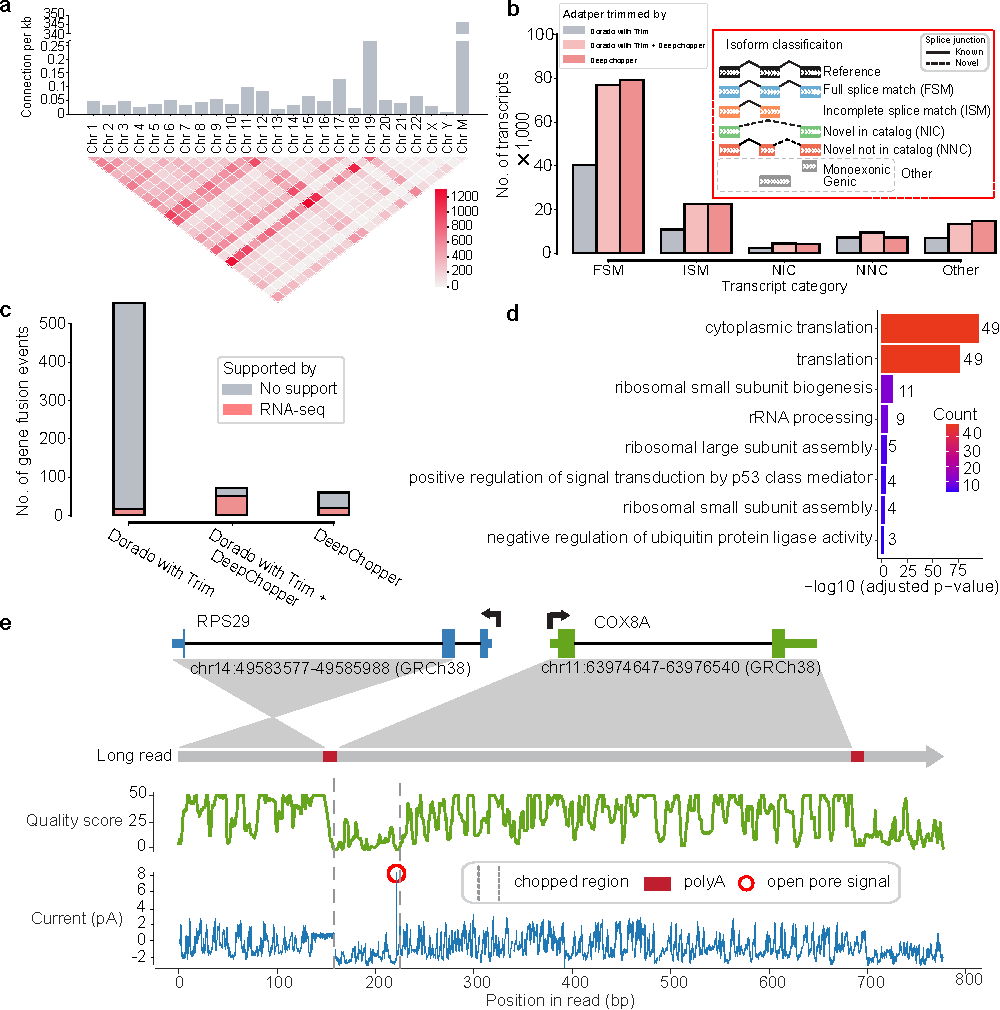
\includegraphics[height=1\columnwidth]{finals/figure3}
	\caption{{\bf Characterization of \gls{drs} chimera artifacts and their impact on downstream analysis in VCaP cells} (a) The upper bar plot shows the number of chimeric connections per kilobase across chromosomes, highlighting higher chimeric activity in Chr 19 and Chr M. The lower heatmap visualizes interchromosomal connections, with intensity indicating the count of connections between different chromosomes. (b) The bar plot shows the number of transcripts (in thousands) across different isoform classification categories. DeepChopper-processed reads result in a higher number of transcripts compared to Dorado-trimmed reads. The inset details the isoform classification scheme. (c) Detected gene fusions from Dorado adapter-trimmed reads and DeepChopper-processed reads. Gene fusions identified from short-read RNA-seq were used to validate fusion events detected from \gls{drs}. (d) \gls{go} enrichment analysis of chimera artifact-affected genes, with color indicating gene count per term. (e) Analysis of a chimeric read artifact detected as an RPS29-COX8A fusion. The schematic shows the fusion between RPS29 (Chr 14) and COX8A (Chr 11). The green plot indicates quality scores along the read, and the blue plot shows raw signal intensity (in pA). The chopped region identified by DeepChopper corresponds to a low-quality segment with low current intensity, polyA, and short open pore signals, suggesting the presence of an \gls{ont} adapter.}\label{fig:f3}
\end{figure}

% % Continuation of the caption on next page
% \begin{figure}[H]
%     \ContinuedFloat
%     \caption{(e) Analysis of a chimeric read artifact detected as an RPS29-COX8A fusion. The schematic shows the fusion between RPS29 (Chr 14) and COX8A (Chr 11). The green plot indicates quality scores along the read, and the blue plot shows raw signal intensity (in pA). The chopped region identified by DeepChopper corresponds to a low-quality segment with low current intensity, polyA, and short open pore signals, suggesting the presence of an \gls{ont} adapter.}
% \end{figure}

\subsection{Impact on Downstream Transcriptome Analysis}

To investigate potential factors contributing to the formation of chimera artifacts, we examined the expression levels and sizes of the genes involved in these artifacts, we found that genes affected by chimera artifacts exhibited significantly higher expression levels compared to all expressed genes (\(\textrm{p-value} < 2.2 \times 10^{-16}\)) (\edfigref{fig:sf4}{a}), while following a similar size distribution pattern (\edfigref{fig:sf4}{b}).
We then analyzed the genomic patterns of improper connections generated by chimera artifacts across chromosomes in VCaP \gls{drs} data.
These artifacts showed varying frequencies across chromosomes, with the mitochondrial chromosome (Chr M) exhibiting an especially high rate of connections per base pair, indicating it may be a hotspot for chimera artifact formation (\figref{fig:f3}{a}).
A similar pattern of improper inter-chromosomal connections was also observed in VCaP RNA004 \gls{drs} data (\edfigref{fig:sf4}{c}), suggesting that chimera artifacts may be an inherent issue of \gls{drs} technology, rather than being fully resolved by improvements in sequencing chemistry.

To evaluate the influence of chimera artifacts on downstream analyses, we investigated the impact of DeepChopper-mediated correction on transcript annotation.
IsoQuant~\cite{prjibelski2023accurate} was employed to detect and annotate transcripts from VCaP \gls{drs} data, focusing on chimeric read artifacts identified by DeepChopper.
By comparing transcript identification with and without DeepChopper correction, we observed an approximately 2-fold increase in the number of identified transcripts (\figref{fig:f3}{b}).
Similar results were also noted for VCaP RNA004 \gls{drs} data (\edfigref{fig:sf4}{d}).
The most prominent increase occurred in the full-length transcripts (\gls{fsm} category), with additional improvements observed across alternatively spliced transcripts (\gls{ism}, \gls{nic}, and \gls{nnc} categories).
These findings underscore the effectiveness of DeepChopper in mitigating the detrimental effects of chimera artifacts on transcript annotation.

Next, we assessed whether DeepChopper could improve gene fusion detection by correcting chimera artifacts. Gene fusion calls identified by FusionSeeker~\cite{chen2023gene} from DeepChopper-processed \gls{drs} reads exhibited an 89\% reduction compared to those detected from Dorado's adapter-trimmed reads.
To further evaluate this reduction, we applied Arriba~\cite{uhrig2021accurate} to detect gene fusions using short-read RNA-seq of VCaP cells and found that none of the gene fusion calls reduced by DeepChopper were supported by those detected in RNA-seq data (\figref{fig:f3}{c}).
This demonstrates that DeepChopper effectively reduces false positive gene fusion calls caused by chimera artifacts in \gls{drs}, an essential improvement for accurately identifying gene fusion drivers in cancer transcriptomes.

Upon closer examination of the chimera artifact-derived gene fusion calls, we found a notable enrichment of ribosomal protein genes (\edfigref{fig:sf5}{a}).
\gls{go} enrichment analysis in VCaP (\figref{fig:f3}{d}) and \gls{sgnex} cell lines (\edfigref{fig:sf5}{b}) confirmed that housekeeping ribosomal protein genes are frequently involved in these artifacts.
Additionally, ribosomal protein genes were also enriched in the chimera artifacts associated with RNA004 chemistry (\edfigref{fig:sf5}{b}).
A manual inspection of a chimeric read identified as an RPS29-COX8A fusion, involving the 40S ribosomal protein S29 in VCaP \gls{drs} data, revealed that the DeepChopper-processed region aligned with raw current signals showing low intensity, indicative of \gls{ont} adapters (\figref{fig:f3}{e}).
The presence of polyA and open pore signals at the boundary of this region further suggested that this chimeric read resulted from improperly joined mRNA transcripts, rather than representing a genuine gene fusion event.

In conclusion, DeepChopper demonstrates the effective application of language models in long-read sequence analysis by addressing the previously unrecognized issue of chimera artifacts in nanopore \gls{drs}. By precisely identifying and removing \gls{ont} adapters from base-called long-read sequences, DeepChopper substantially improves \gls{drs} data quality, allowing for more accurate transcript and gene fusion analyses. Beyond its immediate application in enhancing \gls{drs} data integrity, this work establishes a practical framework for applying language models to resolve complex challenges in long-read sequencing technologies. Looking forward, DeepChopper could be adapted to detect additional artifact types or expanded to support other aspects of long-read analysis, ultimately advancing capabilities across diverse research domains.

\section{Methods}\label{sec:methods}

\subsection{Cell culture}

This is a test. VCaP cell line was obtained from the \gls{atcc} and cultured under sterile conditions to maintain optimal growth and viability.
The cells were grown in Dulbecco's Modified Eagle Medium (DMEM, high glucose; Gibco, Cat\# 11-965-092) supplemented with 10\% fetal bovine serum (FBS Opti-Gold, Performance Enhanced, US Origin; Gendepot, Cat\# F0900-050) to provide essential growth factors.
In addition, the culture medium was enriched with \SI{5}{\ml} of 100 mM Sodium Pyruvate (Gendepot, Cat\# CA017-010) to support cellular metabolism and \SI{5}{\ml} of Antibiotics-Antimycotics (\( 100\times \)) (Gendepot, Cat\# CA002-010) to prevent microbial contamination.
Cells were cultured in \SI{100}{\mm} cell culture treated dishes (Thermo Fisher Scientific, Cat\# 12-556-002) and incubated at \SI{37}{\degreeCelsius} in a humidified atmosphere containing 5\% CO2, with media changes performed every 72 hours to ensure nutrient availability and waste removal.
Cell confluency was regularly monitored and subculturing was performed before reaching 80\% confluency to maintain healthy growth conditions and prevent over-confluence stress.

\subsection{RNA extraction and quantification}

Total RNA was extracted using the RNeasy Mini Kit (Qiagen, Cat\# 74104) according to the protocol of the manufacturer.
The quality and concentration of RNA were assessed using an Agilent 2100 Bioanalyzer.
Poly(A)+ RNA was then enriched from total RNA using the Dynabeads\textsuperscript{tm} mRNA Purification Kit (Invitrogen, Cat\# 65001), which utilizes oligo (dT) beads for selective mRNA binding.
The mRNA was quantified using a Qubit 4 fluorometer and a Qubit RNA HS Assay Kit (Thermo Fisher Scientific, Cat\# Q32852).
The mRNA preparations were either immediately used to prepare a sequencing library or frozen and stored at \SI{-80}{\degreeCelsius} until further use.

\subsection{Nanopore sequencing}

We performed nanopore \gls{drs} sequencing of the enriched mRNA using two different sets: the RNA002 kits with R9.4.1 flow cells and the RNA004 kits with R10.4.1 flow cells.
The decision to incorporate the RNA004 kit, a newly released option, was driven by our intention to test its capabilities in conjunction with our DeepChopper tool to optimize data quality and sequencing efficiency.
For the RNA002 library, \SI{1}{\micro\gram} of poly(A)+ RNA was used as input for library preparation using the Direct RNA Sequencing Kit (SQK-RNA002, \gls{ont}) following the manufacturer's instructions.
Nanopore \gls{drs} employs a \gls{rta} that typically binds to the poly(A) tails of \gls{mrna}; subsequently, a sequencing adapter is ligated to the \gls{rta}, which guides the mRNA through the nanopore for sequencing.
The prepared library was loaded onto four MinION R9.4 flow cells (FLO-MIN106) and sequenced for 48 hours using the Oxford Nanopore MinION device.
For the RNA004 library, 300 ng of poly(A)+ RNA was used as input for library preparation using the Direct RNA Sequencing Kit (SQK-RNA004, \gls{ont}) according to the protocol of the manufacturer.
The library was then loaded onto a PromethION RNA Flow Cell (FLO-PRO004RA) and sequenced on the Oxford Nanopore PromethION device for 72 hours.

For Direct cDNA sequencing, we utilized the Direct cDNA Sequencing Kit (SQK-DCS109, \gls{ont}) following the manufacturer's protocol.
Briefly, \SI{5}{\micro\gram}  of total RNA was used as input for first-strand cDNA synthesis using Maxima H Minus Reverse Transcriptase (Thermo Fisher Scientific) with the SSP and VN primers provided in the kit.
To eliminate potential RNA contamination, we treated the sample with RNase Cocktail Enzyme Mix (Thermo Fisher Scientific).
Second-strand cDNA synthesis was carried out using LongAmp Taq Master Mix (New England Biolabs).
The resulting double-stranded cDNA underwent end-repair and dA-tailing using the NEBNext Ultra End Repair/dA-Tailing Module (New England Biolabs).
Subsequently, sequencing adapters were ligated to the prepared cDNA using Blunt/TA Ligase Master Mix (New England Biolabs).
Between each enzymatic step, the cDNA and libraries were purified using AMPure XP beads (Agencourt, Beckman Coulter).
We quantified the libraries using a Qubit Fluorometer 3.0 (Life Technologies) to ensure adequate concentration and quality.
The final library was loaded onto a MinION R9.4 flow cell and sequenced on the Oxford Nanopore MinION device for 72 hours.

\subsection{Training data preparation}\label{ssec:data}

We acquired \gls{ont} \gls{drs} FAST5 data from the \gls{sgnex} project, which includes six human cell lines: HEK293T, A549, K562, HepG2, MCF7, and HCT116~\cite{chen2021systematic}.
The FAST5 files were converted to POD5 format using the POD5 conversion tool (\url{https://pod5-file-format.readthedocs.io}).
Subsequently, FASTQ files were generated using Dorado (v0.5.2)~\cite{dorado2023} with adapter trimming disabled (\texttt{--no-trim}) and the ``rna002\_70bps\_hac@v3'' model.
The reads were then aligned to the human reference genome (GRCh38) using minimap2 (v2.24)~\cite{li2018minimap2} with ONT direct RNA-specific parameters (-ax splice -uf -k14) for optimized alignment. The resulting SAM files were then converted to BAM format, indexed, and sorted using SAMtools (v1.19.2)~\cite{li2009sequence}.

\hl{For adapter sequence extraction, we selected primary alignments without supplementary alignments and implemented a refined identification protocol. While $3'$ end soft-clipped regions were candidates for adapter sequences, we did not assume all such regions corresponded to adapters.
	Instead, we incorporated a critical biological refinement step: we first identified polyA tails at the beginning of soft-clipped regions, as these represent reliable biological indicators of transcript termination.
	Only sequences following these polyA tails were designated as potential adapter sequences, while aligned regions were classified as non-adapter sequences.
	This approach significantly improved the precision of our training data by distinguishing true adapter sequences from other non-adapter soft-clipped regions that might result from alignment artifacts or sequencing errors.
	By anchoring our adapter identification to known biological features, we reduced the risk of misclassification and ensured the training data more accurately reflected the natural transcript-adapter boundaries encountered in direct RNA sequencing.}

To create artificial chimeric reads, we randomly combined two non-adapter sequences with one adapter sequence to create FASTQ records.
The dataset consists of positive examples containing adapter sequences (with a 1:1 ratio of $3'$ end and internal adapters) and negative examples without any adapter sequences, in a 9:1 ratio.
In total, 600,000 data points were generated and divided into training ($N=480,000$), validation ($N=60,000$), and test sets ($N=60,000$) in an 8:1:1 ratio using stratified random sampling.

\subsection{Language model architecture}\label{ssec:lm}

DeepChopper approaches adapter sequence identification as a token classification task, utilizing a model with 4.6 million trainable parameters.
The system tokenizes biological sequences at single-nucleotide resolution, with each nucleotide (\emph{A}, \emph{C}, \emph{G}, \emph{T}, and \emph{N}) serving as a fundamental token.
This nucleotide-level granularity enables precise discrimination between artificial adapter sequences and native biological sequences.

At its core, DeepChopper employs HyenaDNA~\cite{nguyen2024hyenadna} as its primary feature extractor.
HyenaDNA processes the input sequence using multiple attention-free linear layers with a receptive field, transforming the nucleotide tokens into rich 256-dimensional feature representations.
The model handles variable-length sequences through a padding approach, maintaining consistent performance across different sequence lengths while efficiently capturing long-range dependencies.

These features are then fed through a quality block that incorporates standardized base quality scores.
Prior to processing, the quality scores are normalized using z-score standardization ($\mu=0$, $\sigma=1$) to ensure numerical stability.
The quality block, comprising two \glspl{mlp} with residual connections (hidden dimensions: 256), processes this normalized quality information while preserving the original sequence features.
Each \gls{mlp} layer is followed by ReLU activation, enhancing the model's ability to learn complex quality-sequence relationships.

\hl{The processed sequence features are subsequently fed into a classification head consisting of a two-layer neural network. This architecture transforms the feature representations into classification outputs at the nucleotide level. The classification module employs a softmax activation function to compute probability distributions across two classes: adapter and non-adapter.
	For a given nucleotide position with output logits $z_1$ and $z_2$ (corresponding to adapter and non-adapter classes), the softmax function computes class probabilities as:}

\[ P(y_i=c) = \frac{e^{z_c}}{\sum_{j=1}^{2} e^{z_j}} \]

\hl{where $P(y_i=c)$ represents the probability that nucleotide position $i$ belongs to class $c$.
	The final classification decision is based on the class with the higher probability score.
	In other words, a nucleotide is classified as an adapter if $P(y_i = \textrm{adapter}) > P(y_i = \textrm{non-adapter})$.}

\hl{This position-wise classification approach enables precise identification of adapter sequences at both terminal and internal positions within reads. By performing fine-grained nucleotide-level classification, DeepChopper accurately defines adapter boundaries, facilitating effective trimming across diverse \mbox{\gls{drs}} datasets.}

\subsection{Model training}\label{ssec:training}


DeepChopper processes sequences up to 32,770 nucleotides in length, excluding any longer sequences from analysis.
To ensure efficient batch processing, shorter sequences were padded to this maximum length.
The model was trained using a supervised learning approach, utilizing sequences labeled with adapter annotations.
Training was performed in a \gls{hpc} cluster using two A100 \glspl{gpu}.
The batch size was set to 64, and validation was performed every 20,000 steps.
The model with the highest validation F1 score for the base prediction task was selected for subsequent analyses.
Training was carried out over \num{60} epochs, with early stopping applied based on validation performance to mitigate overfitting risks.

The Adam optimizer was used for parameter optimization, with settings of \(\beta_{1} = 0.9 \) and \(\beta_{2} = 0.999 \)~\cite{kingma2014adam}.
A learning rate scheduler was used to reduce the learning rate when validation loss ceased improving, starting with an initial learning rate of \(2 \times 10^{-5} \).
The cross-entropy loss function was used to update the model parameters, defined as follows:
\[
	\mathcal{L}_{\textrm{BCE}} = -\frac{1}{N} \sum_{i=1}^{N} [y_i \log(\hat{y}_i) + (1 - y_i) \log(1 - \hat{y}_i)]
\]
where \(\mathcal{L}_{\textrm{BCE}}\) is the binary cross-entropy loss, \(N\) is the total number of tokens in the input sequence, \(y_i\) is the ground true label for the \(i\)-th token, and \(\hat{y}_i\) is the predicted probability for the \(i\)-th token.

The average cross-entropy loss across the mini-batch is computed as:
\[
	\mathcal{L}_{\textrm{BatchBCE}} = \frac{1}{B} \sum_{j=1}^{B} \mathcal{L}_{\textrm{BCE}}(\mathbf{y}_j, \hat{\mathbf{y}}_j)
\]
where \(\mathcal{L}_{\textrm{BatchBCE}}\) is the average binary cross-entropy loss for the mini-batch, \(B\) is the batch size (number of sequences in the mini-batch),  and \(\mathbf{y}_j\) and \(\hat{\mathbf{y}}_j\) are the true labels and predicted probabilities for the \(j\)-th sequence in the batch.

The model evaluation metrics included accuracy, precision, recall and the F1 score, calculated using the following equations:
\begin{align*}
	\textrm{Precision} & = \frac{\textrm{TP}}{\textrm{TP}+\textrm{FP}}                                                     \\
	\textrm{Recall}    & = \frac{\textrm{TP}}{\textrm{TP}+\textrm{FN}}                                                     \\
	\textrm{F1}        & = 2 \times \frac{\textrm{Precision} \times \textrm{Recall}}{\textrm{Precision} + \textrm{Recall}}
\end{align*}

The final selection of the model was based on the optimal performance in the validation set.
The model is implemented by PyTorch (v2.5.0)~\cite{paszke2019pytorch}.
To identify the best hyperparameter configuration, the Hydra (v1.3.2)~\cite{Yadan2019Hydra} framework was used.

	% For the specific subsection you want to highlight:
	{
		\titleformat{\subsection}
		{\normalfont\large\bfseries}
		{\thesubsection}
		{1em}
		{\colorbox{yellow}}  % This highlights the subsection title

		\subsection{Ablation Study of Quality Block Component}
	}

\hl{To evaluate the contribution of the quality block to our model's performance, we conducted an ablation study comparing two model configurations: one with the quality block and one without.
	Both model variants were trained using the same training strategy as described previously in \mbox{\hyperref[ssec:data]{Training data preparation}} and \mbox{\hyperref[ssec:training]{Model trainnnig}}, but with a dataset consisting of 100,000 samples in total.
	The training procedure maintained consistent hyperparameters across both configurations, including learning rate, batch size, and optimization algorithm.
	The only difference between the two models was the presence or absence of the quality block component.
	Performance was evaluated using the F1 score metric on a held-out test set.}


\subsection{Sliding window approach for prediction refinement}

To improve the accuracy and smoothness of the predictions, a sliding window approach was implemented.
This method extends the predicted regions and minimizes noisy predictions, aligning with the typical length of adapter sequences observed in the \gls{ont} \gls{drs} data.
The sliding window strategy effectively maintains continuity in regions predicted to contain adapter sequences, preventing fragmented and unrealistic results.

A sliding window size of 21 nucleotides was selected based on empirical optimization, balancing the need for smoothing while retaining sensitivity to shorter adapter sequences.
Within each window, a voting mechanism was applied to refine the predictions.
The final classification $y_i$ for each nucleotide \( x_i \) was determined by the majority vote of all predictions within the window, as defined by the following equation:
\[
	y_i = \begin{cases}
		1 & \text{if } \sum_{j=i-k}^{i+k} p_j > \frac{W}{2} \\
		0 & \text{otherwise}
	\end{cases}
\]
where \(y_i\) is the final prediction for the $i$-th nucleotide, \( W \) is the sliding window size, \( k \) is half the window size (\( k = \frac{W-1}{2}\)), and  \(p_j\) represents the initial predicted label for the \(j\)-th nucleotide within the window, where a value of 1 indicates that the nucleotide is part of an adapter sequence, and a value of 0 indicates that it is part of a non-adapter sequence.

The combination of the sliding window technique and voting-based refinement significantly improved prediction accuracy by smoothing the outputs and reducing false positives, resulting in more reliable data essential for downstream analysis.

\subsection{Post-processing and filtering}

After refining the adapter predictions, four filtering steps were applied to enhance the quality of the final results:
\vspace{.5em}
\begin{enumerate}[leftmargin=2em]
	\item A predicted adapter sequence must be at least 13 nucleotides long. Sequences shorter than this length threshold are not considered valid adapters.
	\item If a read contains more than four adapter sequences, the entire read sequence is retained without any adapter removal.
	\item For reads containing four or fewer adapter sequences, the identified adapters are removed and the read is divided into smaller segments.
	\item Any segments resulting from this process that are less than 20 nucleotides long are discarded.
\end{enumerate}
\vspace{.5em}
Each remaining segment and its corresponding base quality scores are stored as a single read record in the final FASTQ file.
This filtering process separates chimeric read artifacts containing internal adapters into multiple segments, while retaining reads with $3'$ end adapters as single shortened segments.

\subsection{BLAT identity calculation}

The accuracy of DeepChopper in detecting adapter sequences was evaluated by aligning the identified sequences to the human reference genome using \gls{blat}~\cite{kent2002blat}.
A \gls{blat} identity score was defined as the ratio of matched bases to the total sequence length:
\[
	\textrm{BLAT Identity} = \frac{\textrm{Match Length}}{\textrm{Sequence Length}}
\]
In this context, match length refers to the number of bases in the query sequence that align with the reference genome, while sequence length denotes the total length of the query sequence.
This score provides a quantitative measure of how closely each identified sequence aligns with the reference genome, serving as an indicator of detection accuracy.
The alignments were performed using the PxBLAT (v1.2.1)~\cite{li2024pxblat}


% For the specific subsection you want to highlight:
{
	\titleformat{\subsection}
	{\normalfont\large\bfseries}
	{\thesubsection}
	{1em}
	{\colorbox{yellow}}  % This highlights the subsection title

	\subsection{Computational benchmarks}
}

\hl{All benchmarks were conducted in triplicate using btop (\mbox{\url{https://github.com/aristocratos/btop}}, v1.4.0) and nvtop (\mbox{\url{https://github.com/Syllo/nvtop}}, v3.1.0) to monitor CPU and GPU memory usage, respectively. Evaluations were performed on high-performance computing infrastructure with 16 CPU cores, 60 GB RAM, and dual NVIDIA A100 GPUs (80 GB memory each). Adapter prediction stage used a batch size of 64.}


% 24 25 26
% 4:26  3:41 3:40
% 51 58 56
\subsection{Validation of chimera artifact reduction}

Cross-platform validation of \gls{drs} chimera artifacts identified by DeepChopper was conducted leveraging \gls{ont} direct cDNA sequencing and additional cDNA-based sequencing platforms.
Direct cDNA sequencing validation was performed using six cancer cell lines, including the VCaP dataset generated in this study and five published datasets (A549, K562, HepG2, MCF7, and HCT116) obtained from the \gls{sgnex} project~\cite{chen2021systematic}.
The direct cDNA data in FAST5 format were converted to POD5 format using the POD5 conversion tool (\url{https://pod5-file-format.readthedocs.io}).
Subsequently, FASTQ files were generated using Dorado (v0.5.2)~\cite{dorado2023} with adapter trimming enabled (\texttt{--trim} adapters) and the ``dna\_r9.4.1\_e8\_hac@v3.3'' model.
The reads were then processed using Pychopper (\url{https://github.com/epi2me-labs/pychopper}, v2.7.9) and Cutadapt (v4.2)~\cite{martin2011cutadapt} according to a published protocol~\cite{grunberger2022nanopore}.
The oriented reads were aligned to the human reference genome (GRCh38) using minimap2 (v2.24)~\cite{li2018minimap2} with optimized parameters (-ax splice -uf -k14) for spliced alignment.
The resulting SAM files were then converted to BAM format, indexed, and sorted using SAMtools (v1.19.2)~\cite{li2009sequence}.

Additional cDNA-based long-read sequencing data from the WTC11 (human) and F121-9 (mouse) cell lines were used for further validation, incorporating five distinct platforms: \gls{ont} \gls{pcr}-cDNA, \gls{ont} CapTrap, \gls{ont} R2C2, \gls{pb} cDNA, and \gls{pb} CapTrap.
The raw FASTQ files (and FASTA files for \gls{ont} R2C2) from these datasets were provided by the \gls{lrgasp} project~\cite{pardo2024systematic}.
For the \gls{pcr}-cDNA data, the reads were processed using Pychopper (\url{https://github.com/epi2me-labs/pychopper}, v2.7.9) and Cutadapt (v4.2)~\cite{martin2011cutadapt}, following the protocol described in reference~\cite{grunberger2022nanopore}. \gls{ont} reads were then aligned to the human reference genome (GRCh38) or mouse reference genome (GRCm39) using minimap2 (v2.24)~\cite{li2018minimap2} with the parameters (-ax splice -uf -k14), while \gls{pb} reads were aligned using the parameters (-ax splice:hq -uf).
The \gls{ont} \gls{drs} data from A549, K562, HepG2, MCF7, HCT116, VCaP, WTC11 and F121-9 cell lines were processed as previously described, except that The F121-9 cell line data was aligned to the mouse reference genome (GRCm39).

To validate the chimeric alignments derived from \gls{drs}, comparisons were made with chimeric alignments identified from cDNA-based data across the specified platforms.
Chimeric alignments, defined by a primary alignment and one or more supplementary alignments, each containing the SA tag in the BAM file, were converted into lists of genomic intervals based on their corresponding alignments.
The genomic interval lists were then compared between platforms, and overlapping intervals were considered concordant if the distance difference between them was less than 1000 bp.
Supporting rates were calculated as the proportion of \gls{drs} chimeric alignments corroborated by cDNA-based platforms, thereby providing cross-validation of chimera artifacts identified by DeepChopper.

% Sequences longer than 20 bp were aligned to the reference genome using \gls{blat}.
% The resulting identity scores were used to distinguish between true biological sequences and potential chimeric reads, with lower scores indicating likely artificial sequences.
% To evaluate terminal artificial sequences, we employed the \gls{blat} identity threshold of 0.9 to classify hits and non-hits.
% To assess DeepChopper's accuracy in detecting terminal artificial sequences, we compared its predictions to the soft-clipped regions in untrimmed Dorado-processed data.
% An overlap threshold of 0.4 was used to determine the concordance between the two methods.

\subsection{Gene expression analysis and transcript classification}

Gene expression levels from \gls{drs} were quantified using IsoQuant (v3.1.2)~\cite{prjibelski2023accurate}, with the parameters (\texttt{--}data\_type nanopore \texttt{--}stranded forward \texttt{--}model\_construction\_strategy default\_ont \texttt{--}sqanti\_output). The ``\texttt{--}sqanti\_output'' option enables IsoQuant to generate files containing transcript classification information, analogous to the output provided by SQANTI~\cite{tardaguila2018sqanti}.


\subsection{Gene fusion identification and visualization}

For \gls{ont} \gls{drs} data, gene fusions were identified using FusionSeeker (v1.0.1)~\cite{chen2023gene} with default settings.
For short-read RNA-seq data, FASTQ files for the VCaP cell line were obtained from the \gls{ccle} project~\cite{barretina2012cancer} under SRA accession SRX5417211.
Raw reads were mapped to the hg38 reference genome using STAR (v2.7.11)~\cite{dobin2013star}, and gene fusion events were detected with Arriba (v2.4.0)~\cite{uhrig2021accurate}.
The gene structure of the RPS29-COX8A fusion was visualized using GSDS (v2.0)~\cite{hu2015gsds}.
Base quality scores were generated with a custom Python script, and ion current signals were visualized using Squigualiser (v0.6.3)~\cite{samarakoon2024interactive}.
The circos plot for gene fusion events was visualized using chimeraviz (v1.30.0)~\cite{laagstad2017chimeraviz}.

\subsection{GO enrichment analysis}

\gls{go} enrichment analysis of biological processes for genes involved in chimera artifacts identified in \gls{drs} data was performed using the \gls{david} webserver~\cite{sherman2022david}.

\subsection{Computing resource}

All computations were performed on a \gls{hpc} server equipped with a 64-core Intel(R) Xeon(R) Gold 6338 CPU and 256 GB of RAM. The server was also configured with two NVIDIA A100 \glspl{gpu}, each with 80 GB of memory, enabling efficient processing of both CPU-intensive tasks and \gls{gpu}-accelerated deep learning workloads.

% \section{Tables}\label{sec5}

% Tables can be inserted via the normal table and tabular environment. To put
% footnotes inside tables you should use \verb+\footnotetext[]{...}+ tag.
% The footnote appears just below the table itself (refer Tables~\ref{tab1} and \ref{tab2}).
% For the corresponding footnotemark use \verb+\footnotemark[...]+

% \begin{table}[h]
% \caption{Caption text}\label{tab1}%
% \begin{tabular}{@{}llll@{}}
% \toprule
% Column 1 & Column 2  & Column 3 & Column 4\\
% \midrule
% row 1    & data 1   & data 2  & data 3  \\
% row 2    & data 4   & data 5\footnotemark[1]  & data 6  \\
% row 3    & data 7   & data 8  & data 9\footnotemark[2]  \\
% \botrule
% \end{tabular}

% \footnotetext{Source: This is an example of table footnote. This is an example of table footnote.}
% \footnotetext[1]{Example for a first table footnote. This is an example of table footnote.}
% \footnotetext[2]{Example for a second table footnote. This is an example of table footnote.}
% \end{table}

% \begin{table}[h]
% 	\caption{Benchmarking for different models}
% 	\label{tab:bechmark}
% 	\begin{tabular}{@{}
% 			l
% 			S[table-format=1.4e-2] % Formats the F1 column in scientific notation
% 			S[table-format=1.4e-2] % Formats the Loss column in scientific notation
% 			@{}}
% 		\toprule
% 		{Model}             & {F1}                         & {Loss}                         \\ \midrule
% 		CNN                 & 0.9909037351608276           & 0.00302332011051476            \\
% 		Model with Hyena    & 0.9925663471221924           & 0.002182388212531805           \\
% 		Model with Caduceus & \bfseries 0.9977396130561829 & \bfseries 0.000541145505849272 \\ \bottomrule
% 	\end{tabular}
% 	% \footnotetext{Source: This is an example of table footnote. This is an example of table footnote.}
% 	% \footnotetext[1]{Example for a first table footnote. This is an example of table footnote.}
% 	% \footnotetext[2]{Example for a second table footnote. This is an example of table footnote.}
% \end{table}

\bmhead{Data Availability}

Raw and processed data generated in this study, including \gls{drs} using the SQK-RNA002 and SQK-RNA004 kits, as well as direct cDNA sequencing of VCaP cells, have been deposited in the \gls{geo} under the accession number GSE277934.
A secure token (sdwfckwmbzqdbyx) has been provided for reviewers to access the deposited data.

\bmhead{Code Availability}

DeepChopper, implemented in Rust and Python, is open source and available on GitHub (\url{https://github.com/ylab-hi/DeepChopper}) under the Apache License, Version 2.0.
The package can be installed via PyPI (\url{https://pypi.org/project/deepchopper/}) using pip, with wheel distributions provided for Windows, Linux, and macOS to ensure easy cross-platform installation.
An interactive demo is available on Hugging Face (\url{https://huggingface.co/spaces/yangliz5/deepchopper}), allowing users to test DeepChopper's functionality without local installation.
For large-scale analyses, we recommend using DeepChopper on systems with \gls{gpu} acceleration. Detailed system requirements and optimization guidelines are available in the repository's documentation.

\bmhead{Acknowledgements}

This project was supported in part by NIH grants R35GM142441 and R01CA259388 awarded to RY, and NIH grants R01CA256741, R01CA278832, and R01CA285684 awarded to QC.

\bmhead{Author Contributions}

YL, TYW and RY designed the study with QC. YL and TYW performed the analysis. QG, YR and XL performed the experiments. YL designed and implemented the model and computational tool. YL, TYW, QG and RY wrote the manuscript. RY supervised this work.

\bmhead{Conflict of interests}

RY has served as an advisor/consultant for Tempus AI, Inc. This relationship is unrelated to and did not influence the research presented in this study.

\backmatter

\begin{appendices}
	\printglossaries
\end{appendices}

\bibliography{sn-bibliography}% common bib file

\newpage

\section{Extended data}

\renewcommand{\figurename}{Extended Data Fig.}
\renewcommand{\tablename}{Extended Data Table}


\begin{table}[htbp]
	\centering
	\caption{Comparison of adapter trimming tools}
	\begin{tabular}{lcccc}
		\toprule
		\textbf{Adapter trimming tool}             & \textbf{\begin{tabular}[c]{@{}c@{}}dRNA-seq\\terminal\\adapter\\trimming\end{tabular}} & \textbf{\begin{tabular}[c]{@{}c@{}}dRNA-seq\\internal\\adapter\\trimming\end{tabular}} & \textbf{\begin{tabular}[c]{@{}c@{}}Trimming existing\\dRNA-seq datasets\\(post-basecalling)\end{tabular}} \\
		\midrule
		Porechop~\cite{Wick2017}                   & \texttimes                                                                             & \texttimes                                                                             & \texttimes                                                                                                \\
		Porechop\_ABI~\cite{bonenfant2023porechop} & \texttimes                                                                             & \texttimes                                                                             & \texttimes                                                                                                \\
		Pychopper~\cite{pychopper}                 & \texttimes                                                                             & \texttimes                                                                             & \texttimes                                                                                                \\
		Dorado~\cite{dorado2023}                   & \checkmark                                                                             & \texttimes                                                                             & \texttimes                                                                                                \\
		DeepChopper                                & \checkmark                                                                             & \checkmark                                                                             & \checkmark                                                                                                \\
		\bottomrule
	\end{tabular}
	\footnotetext{\checkmark~indicates the tool supports this functionality; \texttimes~indicates the tool does not support this functionality.}
	\label{tab:st1}
\end{table}


\begin{table}[ht]
	\centering
	\caption{Ablation Study Results for Quality Block}
	\begin{tabular}{lc}
		\toprule
		\textbf{Model Configuration} & \textbf{F1 Score} \\
		\midrule
		With Quality Block           & \textbf{0.99}     \\
		Without Quality Block        & 0.97              \\
		\bottomrule
	\end{tabular}
	\label{tab:st2}
\end{table}



\begin{figure}[!ht]
	\includegraphics[height=0.4\columnwidth]{finals/sf1}
	\caption{{\bf Performance evaluation in a held-out test dataset showing Recall, Precision, and F1 values for DeepChopper, Pychopper, Porechop, and Porechop\_ABI.}}\label{fig:sf1}
\end{figure}

\begin{figure}[!ht]
	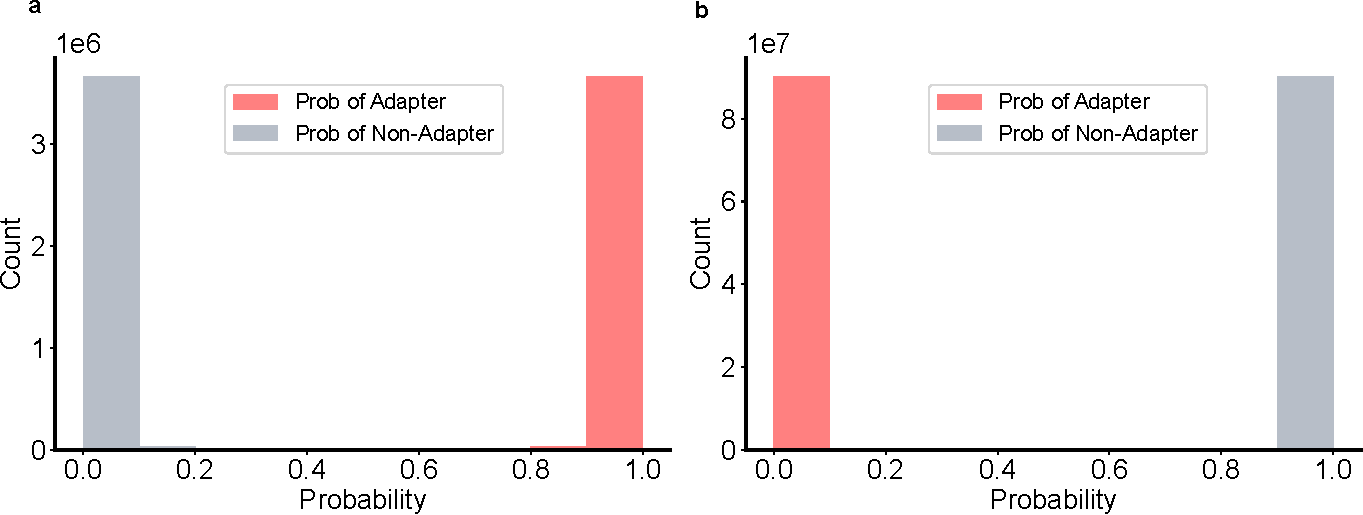
\includegraphics[height=0.35\columnwidth]{finals/adaprob}
	\caption{{\bf Prediction probability distributions of DeepChopper for the held-out test dataset.} (a) Distribution of prediction probabilities for sequences with ground truth adapter classification. Red bars represent the probability of adapter prediction, while gray bars show the probability of non-adapter prediction. The count (y-axis) is shown in millions of sequences ($10^6$ scale). (b) Distribution of prediction probabilities for sequences with ground truth non-adapter classification. Red bars indicate the probability of adapter prediction, while gray bars show the probability of non-adapter prediction. The count (y-axis) is shown in tens of millions of sequences ($10^7$ scale). Both distributions demonstrate strong polarization toward correct classification probabilities, indicating the model's high confidence in distinguishing between adapter and non-adapter sequences.
	}\label{fig:adaprob}
\end{figure}

\begin{figure}[!ht]
	\includegraphics[height=0.4\columnwidth]{finals/sf2a}
	\caption{ {\bf Computational performance metrics across different data sizes from VCaP cell line sequencing.} (a) Runtime analysis showing processing time requirements for different pipeline stages (FASTQ Conversion, Prediction, Post-Processing) and total runtime across four data sizes (0.1M, 0.5M, 1M, and Full dataset (9M)) sampled from the VCaP cell line. As data size increases, prediction time becomes the dominant component, with the full dataset requiring approximately 5 hours of total processing time. (b) Memory usage comparison between CPU and GPU implementations across the same VCaP data sizes. The prediction stage shows consistently higher memory requirements, with CPU memory usage for prediction reaching approximately 70 GB for the larger datasets. All measurements include error bars representing standard deviation from three runs.}\label{fig:sf2a}
\end{figure}


\begin{figure}[!ht]
	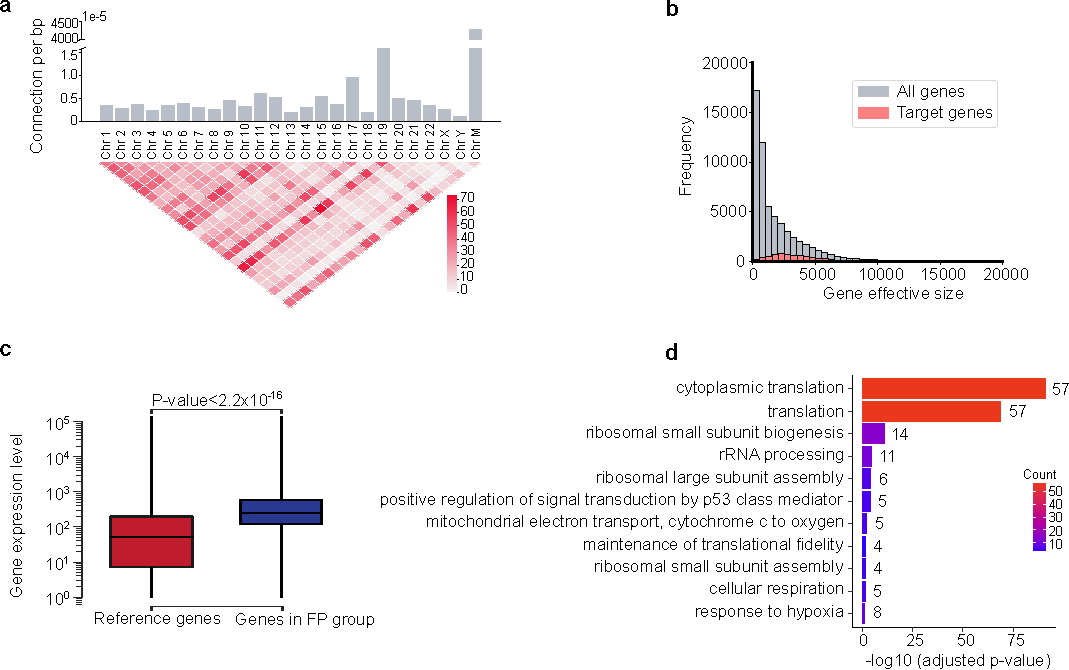
\includegraphics[height=0.21\columnwidth]{finals/sf2}
	\caption{ {\bf Chimeric alignments from \gls{drs} of the F121-9 cell line (mouse), evaluated for support using additional \gls{ont} and \gls{pb} sequencing data with different protocols. DeepChopper reduces unsupported chimeric alignments across all methods compared to Dorado with adapter trimming.}}\label{fig:sf2}
\end{figure}



\begin{figure}[!ht]
	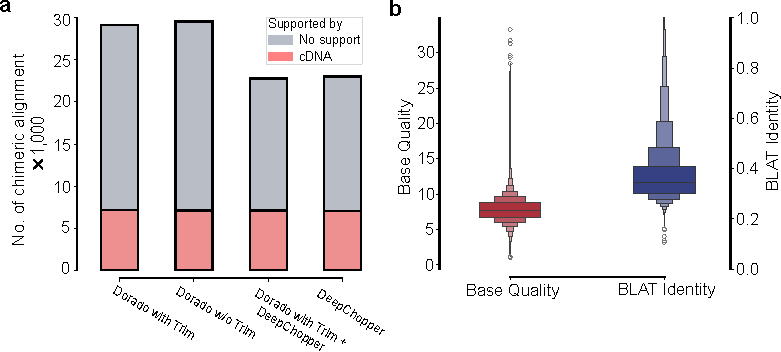
\includegraphics[height=0.41\columnwidth]{finals/sf3}
	\caption{ {\bf Evaluation of DeepChopper's predictions on chimeric read artifacts in \gls{drs} data generated using the SQK-RNA004 kit from the VCaP cell line.} (a) Number of chimeric alignments (in thousands) identified in VCaP RNA004 \gls{drs} reads processed by Dorado with and without adapter trimming, and by DeepChopper. The bar colors indicate chimeric reads supported by cDNA sequencing (red) and those lacking support (grey). (b) Base quality scores (left) and \gls{blat} alignment identity scores (right) for internal adapter sequences identified by DeepChopper in RNA004 \gls{drs} reads.}\label{fig:sf3}
\end{figure}



\begin{figure}[!ht]
	\includegraphics[height=0.65\columnwidth]{finals/sf4}
	\caption{ {\bf Analysis of \gls{drs} chimera artifacts and their genomic and transcriptomic characteristics in VCaP cells.} (a) Box plot comparing gene expression levels between all expressed genes (N=19,156) and genes affected by chimera artifacts (N=7,186) in the VCaP \gls{drs} dataset. Chimera artifacts-affected genes exhibit significantly higher expression levels (\(\textrm{p-value} < 2.2 \times 10^{-16}\)). (b) Distribution of gene effective sizes for all expressed genes and genes affected by chimera artifacts, indicating that the size distributions of genes impacted by chimera artifacts are comparable to those of all expressed genes. (c) Chromosomal distribution and interchromosomal connections from chimeric read artifacts arising from VCaP RNA004 \gls{drs}. The top bar plot shows the number of connections per kilobase for each chromosome, with higher bars indicating more frequent connections. The bottom heatmap visualizes the number of chimeric connections between chromosome pairs, with color intensity representing the connection frequency. (d) Number of detected transcripts across different isoform categories (\gls{fsm}, \gls{ism},  \gls{nic}, \gls{nnc}, and Other) from DeepChopper-identified chimeric read artifacts in VCaP RNA004 \gls{drs} data. DeepChopper-corrected reads resulted in a greater number of transcripts compared to adapter-trimmed reads by Dorado across all categories.}\label{fig:sf4}
\end{figure}


% % First part of the figure
% \begin{figure}[p]
%     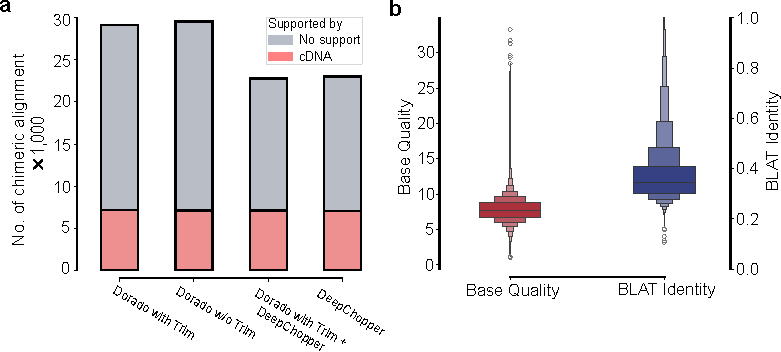
\includegraphics[height=1.4\columnwidth]{finals/sf3}
%     \caption{ {\bf Analysis of gene fusions derived from chimeric read artifacts in \gls{drs}.}}
%     \label{fig:sf3}
% \end{figure}

% % Continuation of the caption on next page
% \begin{figure}[p]
%     \ContinuedFloat
%     \caption{(a) Circos plot depicting chromosomal connections of gene fusions resulting from chimeric read artifacts in VCaP cells. Blue lines represent inter-chromosomal fusion events, while red lines indicate intra-chromosomal fusions. The outer track displays chromosomal ideograms labeled with respective chromosome numbers. (b) \gls{go} enrichment analysis of fusion genes derived from chimeric read artifacts identified by DeepChopper in \gls{drs} data from A549, HepG2, and HCT116 cell lines, and VCaP RNA004 \gls{drs} data. The table lists enriched \gls{go} terms of biological processes, associated genes, and the statistical significance (p-values) for each enrichment.}
% \end{figure}


\begin{figure}[!ht]
	\includegraphics[height=1.45\columnwidth]{finals/sf5}
	\caption{ {\bf Analysis of gene fusions derived from chimeric read artifacts in \gls{drs}.} (a) Circos plot depicting chromosomal connections of gene fusions resulting from chimeric read artifacts in VCaP cells. Blue lines represent inter-chromosomal fusion events, while red lines indicate intra-chromosomal fusions. The outer track displays chromosomal ideograms labeled with respective chromosome numbers. (b) \gls{go} enrichment analysis of fusion genes derived from chimeric read artifacts identified by DeepChopper in \gls{drs} data from A549, HepG2, and HCT116 cell lines, and VCaP RNA004 \gls{drs} data. The table lists enriched \gls{go} terms of biological processes, associated genes, and the statistical significance (p-values) for each enrichment.}\label{fig:sf5}
\end{figure}


% \newpage

% \section{Supplementary information}

% \renewcommand{\figurename}{Supplementary Fig.}
% \renewcommand{\tablename}{Supplementary Table}


% If your article has accompanying supplementary file/s please state so here.
% Authors reporting data from electrophoretic gels and blots should supply the full unprocessed scans for key as part of their Supplementary information. This may be requested by the editorial team/s if it is missing.
% Please refer to Journal-level guidance for any specific requirements.


% \begin{table}
% 	\centering
% 	\caption{Hyperparameter ranges used}\label{tab:hyperparameter}
% 	\begin{tabular}{lc}
% 		\toprule
% 		                     & {$\sf DeepChopper$}               \\
% 		\midrule
% 		Parameters           & 1.6M                              \\
% 		Optimizer            & Adam                             \\
% 		Optimizer momentum   & $\beta_1$, $\beta_2$ = 0.9, 0.999 \\
% 		Training epoch       & 60                                \\
% 		Batch size           & 64                                \\
% 		Learning rate        & 2e-5                     \\
% 		LR scheduler         & ReduceLROnPlateau                 \\
% 		Weight decay (model) & 0                         \\
% 		Sequence lengths     & 32769                             \\
% 		\midrule
% 	\end{tabular}
% \end{table}

% \section*{Declarations}

% Some journals require declarations to be submitted in a standardised format. Please check the Instructions for Authors of the journal to which you are submitting to see if you need to complete this section. If yes, your manuscript must contain the following sections under the heading `Declarations':
%
%\begin{itemize}
%	\item Funding
%	\item Conflict of interest/Competing interests (check journal-specific guidelines for which heading to use)
%	\item Ethics approval and consent to participate
%	\item Consent for publication
%	\item Data availability
%	\item Materials availability
%	\item Code availability
%	\item Author contribution
%\end{itemize}

%
%\begin{appendices}
%	\printglossary[type=\acronymtype, title=Abbreviations]
%
%	\section{Section title of first appendix}\label{secA1}
%
%	An appendix contains supplementary information that is not an essential part of the text itself but which may be helpful in providing a more comprehensive understanding of the research problem or it is information that is too cumbersome to be included in the body of the paper.
%
%	%%=============================================%%
%	%% For submissions to Nature Portfolio Journals%%
%	%% please use the heading ``Extended Data''.   %%
%	%%=============================================%%
%
%	%%=============================================================%%
%	%% Sample for another appendix section			               %%
%	%%=============================================================%%
%
%	%% \section{Example of another appendix section}\label{secA2}%
%	%% Appendices may be used for helpful, supporting or essential material that would otherwise
%	%% clutter, break up or be distracting to the text. Appendices can consist of sections, figures,
%	%% tables and equations etc.


%\end{appendices}

%%===========================================================================================%%
%% If you are submitting to one of the Nature Portfolio journals, using the eJP submission   %%
%% system, please include the references within the manuscript file itself. You may do this  %%
%% by copying the reference list from your .bbl file, paste it into the main manuscript .tex %%
%% file, and delete the associated \verb+\bibliography+ commands.                            %%
%%===========================================================================================%%


%% if required, the content of .bbl file can be included here once bbl is generated
%%\input sn-article.bbl

\end{document}
